
\section{\label{sec:The-prototype}The proof of concept}


\subsection{\label{sub:The-attack-scenarios}The attack scenarios modeled in
the prototype}

Our prototype implements two scenarios that illustrate particular
cases of attacks against hypervisors: denial of service and rootkit
activities. In both scenarios defense policies are expressed in the
terms of guarded commands \cite{Dijkstra:1975:Guarded}. Following
\cite{Dolev:2009:SPC:1552309.1552312} guarded commands are a natural
way to express state-based actions. 


\paragraph{Denial Of Service (DOS) }

In general we distinguish between two kinds of denial of service attacks:
\begin{itemize}
\item Local. A VM sends a lot of sensitive requests (e.g. CPUID \url{http://en.wikipedia.org/wiki/CPUID})
to the hypervisor. Handling sensitive (but not provileged) instructions
hypervisors (in particular KVM) gains the execution context, handles
these instructions and passes the control back to the sending VM.
Such context switches starve hypervisor out of computational resources,
see \cite{ddos-cpuid} for more details.
\item Network-based. A VM floods the network with requests starving the
TCP-related resources.
\end{itemize}
At the hypervisor level, our system handles DOS attacks as follows:
at every SM iteration we count the number $NR$ of DOS requests. If
$NR$ exceeds the certain threshold $Threshold$ we suspice a VM to
run an attacker. If $NR$ remains above $Threshold$ during several
SM iterations, we conclude that a DOS attacker continues to operate
and kill the VM running an attacker. If $NR$ becomes very high, exceeding
the threshold $MaxThreshold$ (which is significantly bigger than
$Threshold$) we kill the VM executing an attacker immediately.


\paragraph{Rootkit activities}

Our system detects attempts to modify the contents of the Interrupt
Description Table (IDT) that contains the entries to software interrupt
handlers (also to system calls because a system call is a particular
case of software interrupt). If a party running at some VM tries to
modify the IDT of the corresponding virtual CPU we assume that this
party is malicious and kill the corresponding VM. This is because
hooking the system control flow (in particular interrupt handlers)
is the preparatory stage towards breaching into the hypervisor as
in \cite{intel-systret,defense-rootkit-attacks,Wang:rootkits:2009}.

The guarded commands for handling IDT changes are provided below:

\begin{multline*}
\forall VMID\in VirtualMachineIDs\cdot\\
IDT\_Changed(VMID)\wedge VM\_Rebooted(VMID)\mapsto KillVM(VMID);
\end{multline*}


and for handling of DOS requests: 

\begin{multline*}
\forall VMID\in VirtualMachineIDs\cdot\\
NumOfRequests(VMID,NR)\rightarrow true;\\
NR>Threshold\rightarrow NumOfAttackingIterations(NA);\\
NA>MaxAttackingIterations\rightarrow KillVM(VMID);\\
NA<MaxAttackingIterations\wedge NR>MaxReqThreshold\rightarrow KillVM(VMID)
\end{multline*}


Figure \ref{fig:The-defense-state-machines} provides the state machines
that illustrate both defense policies.

\begin{figure}
\begin{centering}
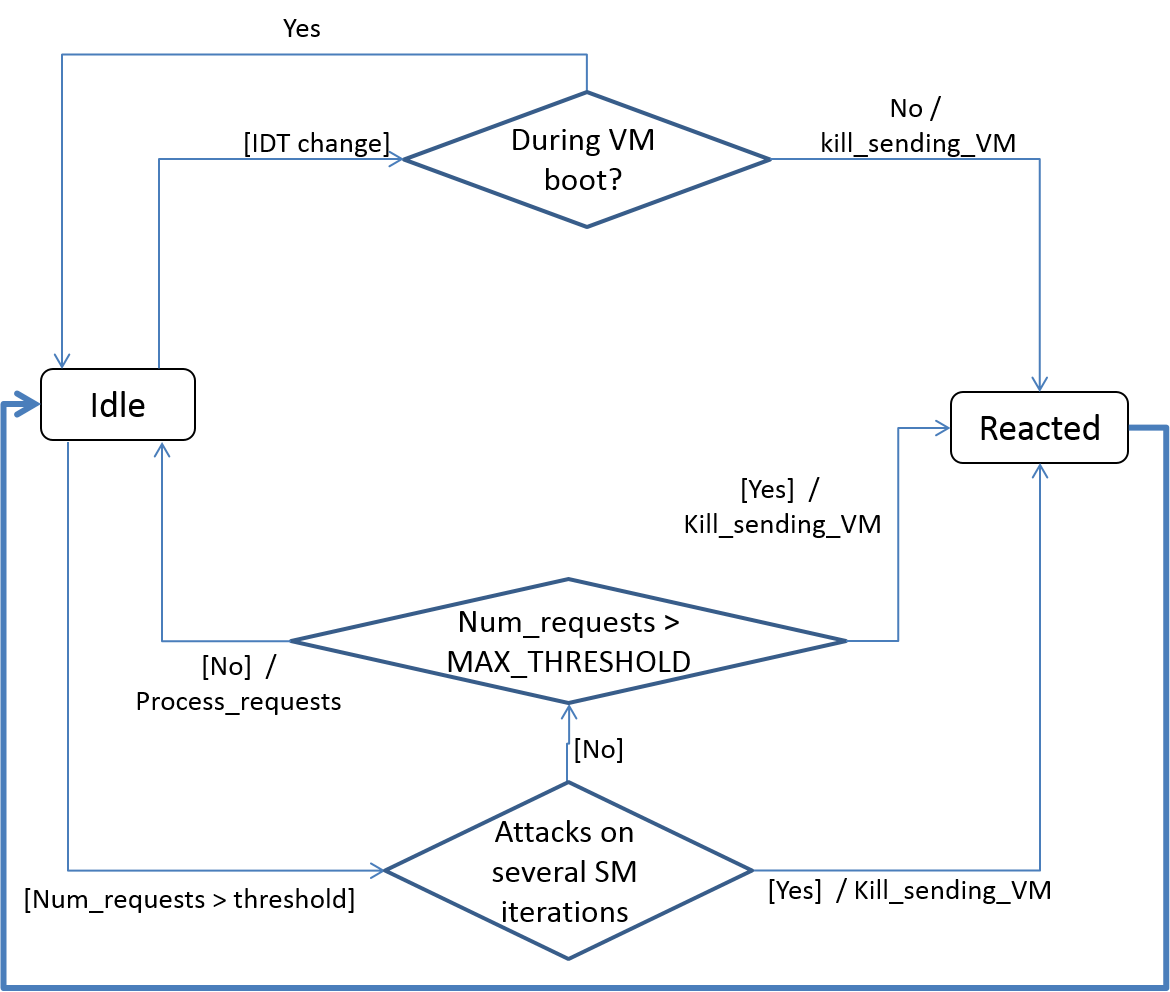
\includegraphics[width=12cm]{pictures/defense-sms}
\par\end{centering}

\caption{\label{fig:The-defense-state-machines}The state machines for the
defense policies implemented in our ptototype}
\end{figure}



\subsection{\label{sub:Implementation-Issues}Implementation Issues}

We are implementing the prototype as a Linux kernel module. Its current
version has the following timer interrupt handlers installed: The
SM timer and the watchdog timer. The SM timer handler does the following:
\begin{itemize}
\item In every execution it checks whether the system state is stable and
in case of need brings the system into a stable state. After these
actions are finished the watchdog timer signal is postponed, thus
illustrating the I'm Alive message.

\begin{itemize}
\item The system state is assumed to be stable if no IDT modifications and
no DDOS attacks are noticed.
\item If the system state is unstable then the SM brings it to a stabe state
as it is described in the previous section , ``The attack scenarios''.
\end{itemize}
\item Once in several executions of the SM timer handler the system state.


The watchdog timer reboots the OS, issuing the Linux system call .

\end{itemize}
We have implemented the first version of the Traffic Monitor. It intercepts
the network traffic between guests, printing out short statistics
about it (e.g., number of bytes). This is done by finding the handlers
for the TCP system calls (i.e., \textsf{sendv}, \textsf{recv}) in
the system call table, following the approach of \cite[Section 7]{pfoh-vmmonitor-2013}.
To make a full-fledged traffic sensor we still have to treat special
cases like the presence of VirtIO infrastructure \cite{VirtIO-Russell}
that consists of special drivers processing I/O at the guest side. 

We are running our prototype on an Intel architecture so we are using
the memory associated with System Management mode (SMM, \cite{GMU-CS-TR-Evasion-2011-8})
to provide the hardware-based write-protection of the Integrity Checker
code. Most of the modern hardware support hardware-based memory protection.
The integrity checker code runs in SMM and is triggered by the hardware
timer. Such a signal is guaranteed to arrive regardless of software
behavior. 

\textcolor{black}{It should be noted that in order to detect rootkits
the whole OS kernel (not just the Stabilization Manager) should be
checked for changes. The inefficiency of this operation is aggravated
by the fact that the Integrity Checker runs it synchronously, freezing
the whole OS. We suggest the following improvement that is supposed
to make the stabilization check more efficient:}
\begin{itemize}
\item \textcolor{black}{Let the Integrity Checker verify the integrity of
the Watchdog solely because the Watchdog module is relatively small.}
\item \textcolor{black}{The Watchdog modulevafter its integrity is confirmed,
launches an asynchronous system state check. }
\end{itemize}
\textcolor{black}{In order to minimize delays caused by the SMM code
execution, extensive system state checks may be carried out at night
time.}
